\documentclass[a4paper,man,natbib]{apa6}

\usepackage{amsmath}
\usepackage{graphicx}
\usepackage[colorinlistoftodos]{todonotes}
\usepackage{epigraph}

\usepackage{pifont}% http://ctan.org/pkg/pifont

\title{Replication of de Vel (2012): Mining Email Content for Author Identification Forensics}
\shorttitle{De Vel Replication}
\author{Marcel Schliebs}
\affiliation{Studienstiftung natur- und ingenieurswissenschaftliches Forschungskolleg}

\abstract{Lorem ipsum pipapo.}

\begin{document}
\maketitle

\section{Introduction}

In this document, I will try to document the process of replication and re-implementation of the algorithm. 


\section{Features}
\label{sec:examples}

Overview over Style Merker Attributes
% latex table generated in R 3.4.1 by xtable 1.8-2 package
% Thu Nov 30 14:36:45 2017
\begin{table}[ht]
\centering
\begin{tabular}{p{1cm}|p{6cm}|p{1cm}|p{3cm}|p{6cm}}
  \hline
 & StyleMarkerAttributeType & Status & VarName & Remarks \\ 
  \hline
1 & Number of blank lines/total number of lines & \ding{51} &  & lorem ipsum pipapo \\ 
  2 & Average sentence length & \ding{51} &  & lalala blablabla \\ 
  3 & Average word length (number of characters) & \ding{51} &  &  \\ 
  4 & Vocabulary richness i.e., V=M & \ding{51} &  &  \\ 
  5 & Total number of function words/M & \ding{51} &  &  \\ 
  6 & Function word frequency distribution (122 features) & \ding{55} &  &  \\ 
  7 & Total number of short words/M & \ding{55} &  &  \\ 
  8 & Count of hapax legomena/M & $\sim$ &  &  \\ 
  9 & Count of hapax legomena/V & $\sim$ &  &  \\ 
  10 & Total number of characters in words/C & \ding{55} &  &  \\ 
  11 & Total number of alphabetic characters in words/C & \ding{51} &  &  \\ 
  12 & Total number of upper-case characters in words/C & $\sim$ &  &  \\ 
  13 & Total number of digit characters in words/C & \ding{51} &  &  \\ 
  14 & Total number of white-space characters/C & \ding{51} &  &  \\ 
  15 & Total number of space characters/C & \ding{51} &  &  \\ 
  16 & Total number of space characters/number white-space characters & \ding{55} &  &  \\ 
  17 & Total number of tab spaces/C & \ding{55} &  &  \\ 
  18 & Total number of tab spaces/number white-space characters & $\sim$ &  &  \\ 
  19 & Total number of punctuations/C & $\sim$ &  &  \\ 
  20 & Word length frequency distribution/M (30 features) & \ding{55} &  &  \\ 
   \hline
\end{tabular}
\end{table}


\subsection{Number of blank lines/total number of lines}


\subsection{Sections}

Use section and subsection commands to organize your document. \LaTeX{} handles all the formatting and numbering automatically. Use ref and label commands for cross-references.

\subsection{Comments}

You can add inline TODO comments with the todonotes package, like this:
\todo[inline, color=green!40]{This is an inline comment.}

\subsection{References}

LaTeX automatically generates a bibliography in the APA style from your .bib file. The citep command generates a formatted citation in parentheses \citep{Lamport1986}. The cite command generates one without parentheses. LaTeX was first discovered by \cite{Lamport1986}.

\subsection{Tables and Figures}

Use the table and tabular commands for basic tables --- see Table~\ref{tab:widgets}, for example. You can upload a figure (JPEG, PNG or PDF) using the files menu. To include it in your document, use the includegraphics command as in the code for Figure~\ref{fig:frog} below.

% Commands to include a figure:
\begin{figure}
\centering
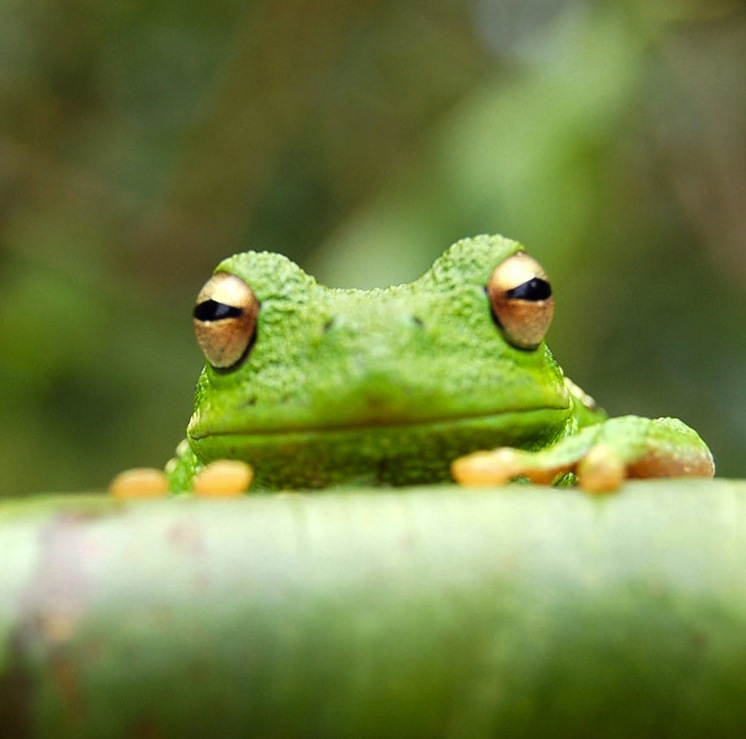
\includegraphics[width=0.5\textwidth]{frog.jpg}
\caption{\label{fig:frog}This is a figure caption.}
\end{figure}

\begin{table}
\centering
\begin{tabular}{l|r}
Item & Quantity \\\hline
Widgets & 42 \\
Gadgets & 13
\end{tabular}
\caption{\label{tab:widgets}An example table.}
\end{table}

\subsection{Mathematics}

\LaTeX{} is great at typesetting mathematics. Let $X_1, X_2, \ldots, X_n$ be a sequence of independent and identically distributed random variables with $\text{E}[X_i] = \mu$ and $\text{Var}[X_i] = \sigma^2 < \infty$, and let
$$S_n = \frac{X_1 + X_2 + \cdots + X_n}{n}
      = \frac{1}{n}\sum_{i}^{n} X_i$$
denote their mean. Then as $n$ approaches infinity, the random variables $\sqrt{n}(S_n - \mu)$ converge in distribution to a normal $\mathcal{N}(0, \sigma^2)$.

\subsection{Lists}

You can make lists with automatic numbering \dots

\begin{enumerate}
\item Like this,
\item and like this.
\end{enumerate}
\dots or bullet points \dots
\begin{itemize}
\item Like this,
\item and like this.
\end{itemize}

We hope you find write\LaTeX\ useful, and please let us know if you have any feedback using the help menu above.

%\bibliography{example}

\end{document}

%
% Please see the package documentation for more information
% on the APA6 document class:
%
% http://www.ctan.org/pkg/apa6
%